\section{Optimal Communication Chain over the Ideal Channel}
\textcolor{red}{[TODO: ADD MORE MATH LATER]}\par
\textcolor{red}{[TODO: MAYBE ADD HOW SOME SIMULATION PARAMETERS AFFECT THE SIMULATION (like taps for example)]}\par
\textcolor{red}{[TODO: MAKE THE AXIS NUMBER OF THE GRAPHS BIGGER]}\par

\subsection{Communication Chain}
\begin{figure}[H]
	\centering
	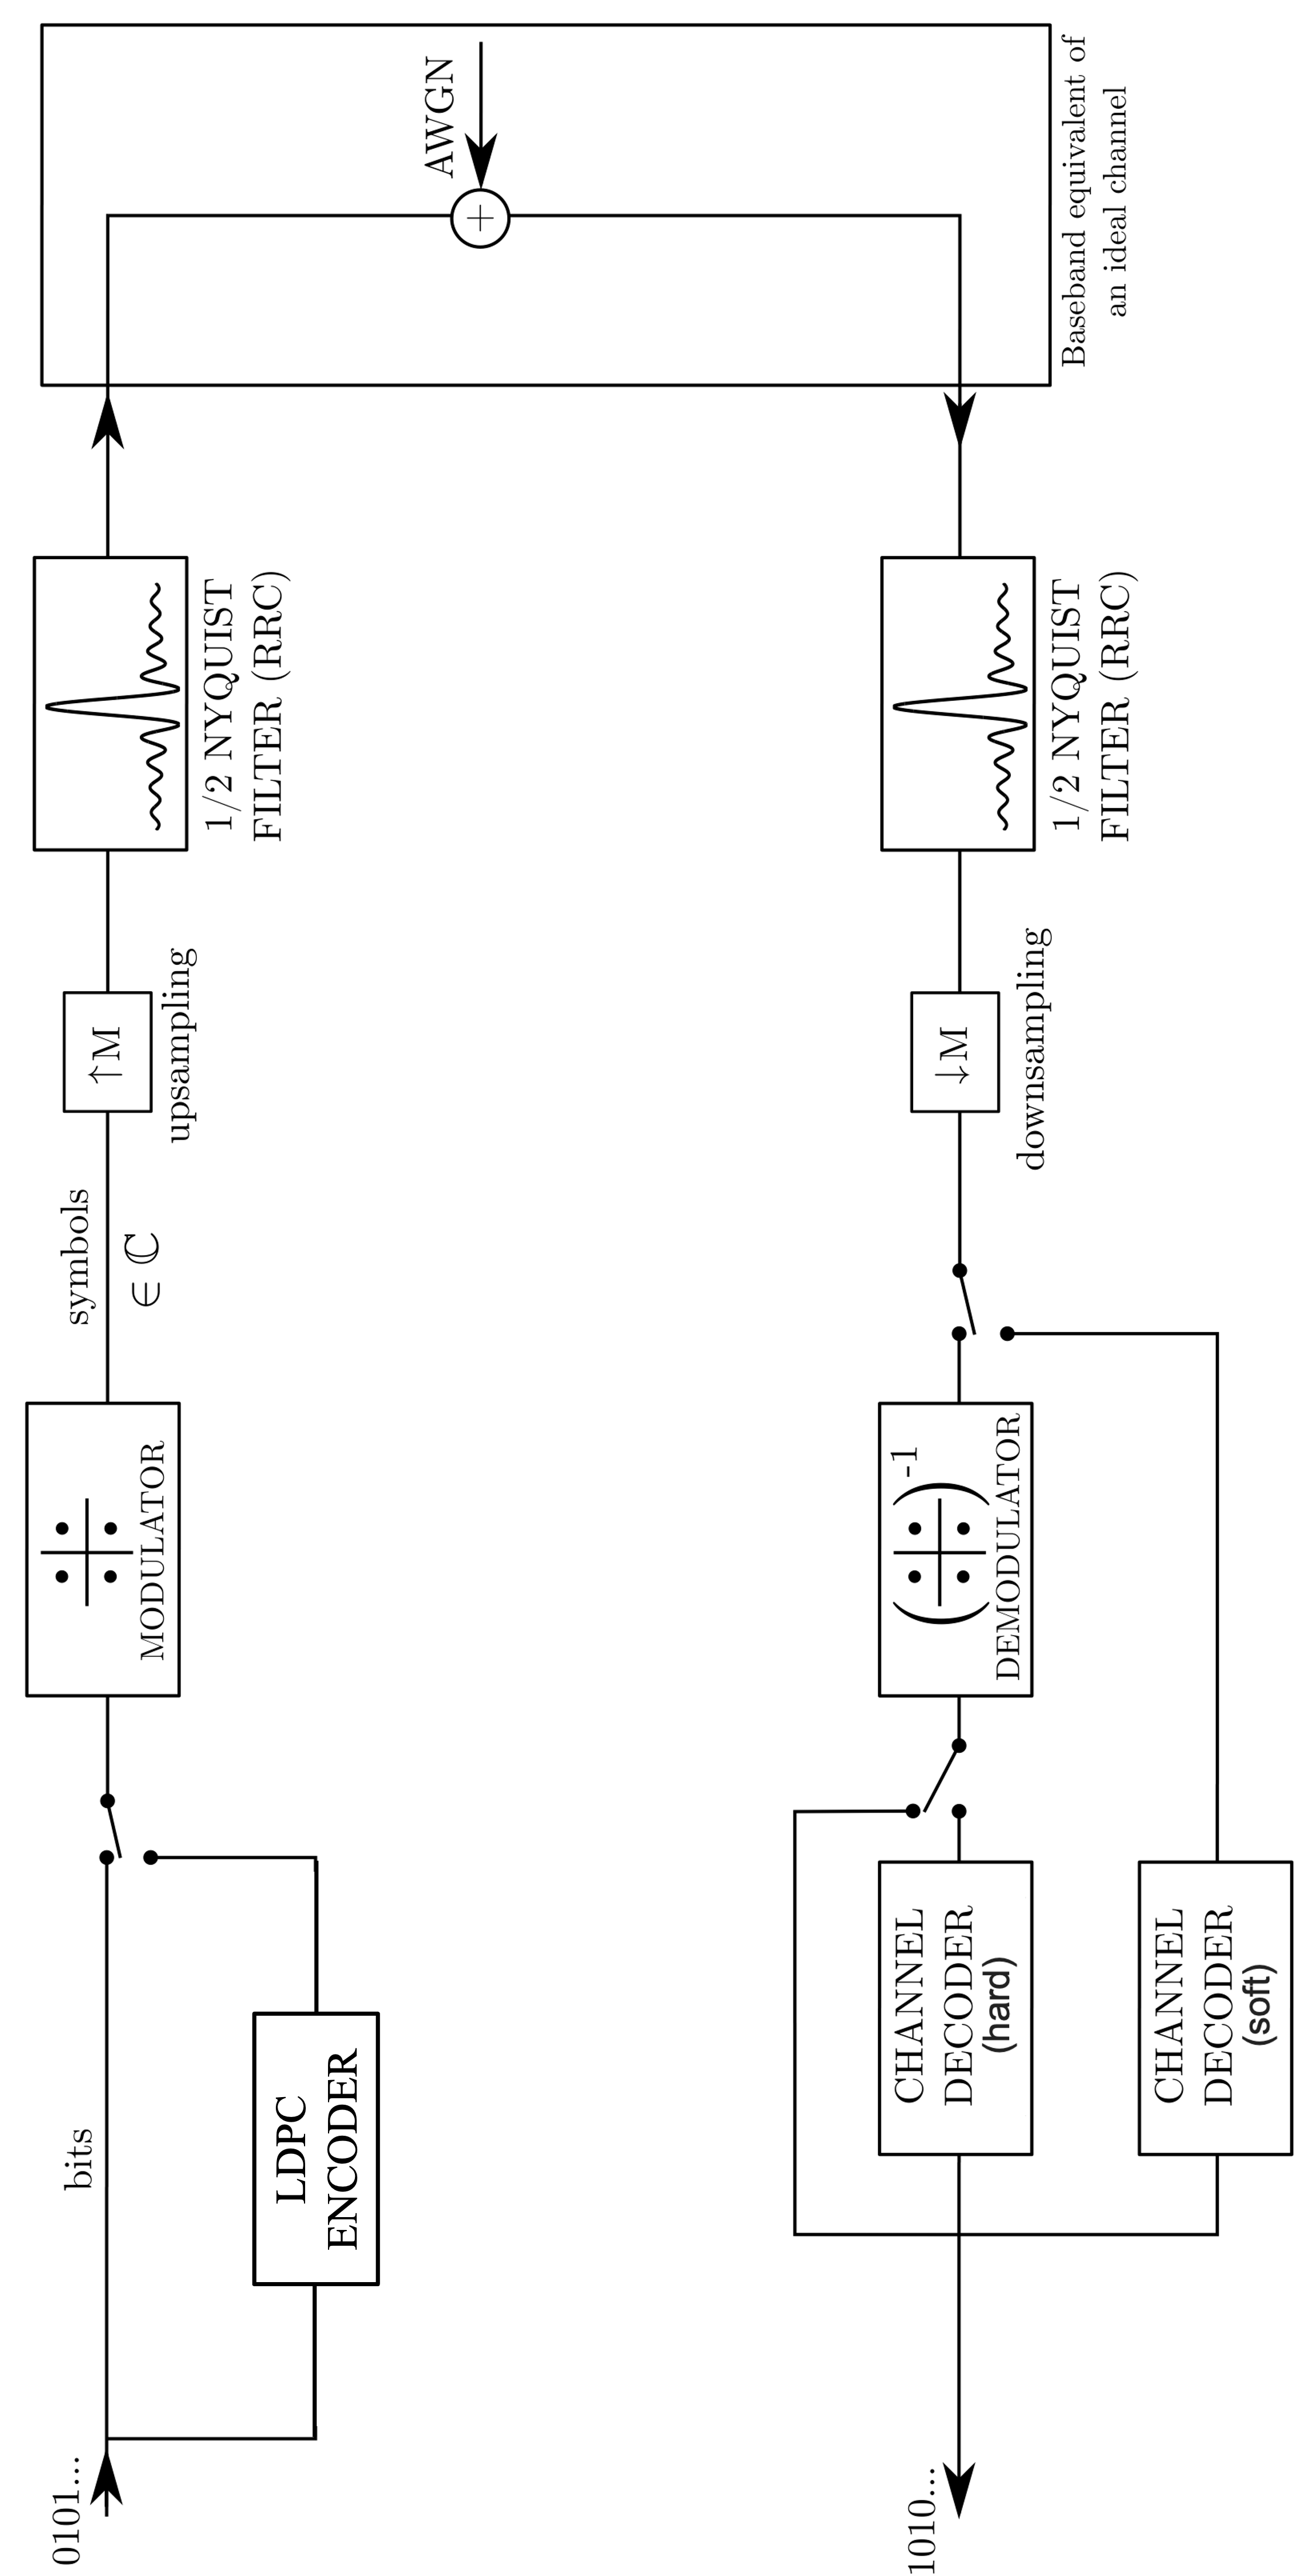
\includegraphics[angle=-90, width=0.9\linewidth]{Images/com-chain} % Ensure 'Images/com-chain' path is correct
	\caption{Block diagram of the communication system}
	\label{fig:com-chain}
\end{figure}
The communication chain depicted in Figure \ref{fig:com-chain} models the pipeline of a DVB-C transmitter and receiver at baseband. On the transmitter side, a bit-stream is generated, then mapped to complex symbols from a chosen QAM modulation. These symbols are subsequently up-sampled and shaped by a half-root Nyquist filter to limit their bandwidth. On the receiver's side, the transmitted signal is matched-filtered with the same half-root Nyquist filter to maximize the signal-to-noise ratio. The output of the matched filter is then down-sampled at the symbol instances and demapped to recover an estimate of the transmitted bit-stream.\\
In this project, the Low Density Parity Check Encoder is not implemented, and the algorithms for symbol mapping and demapping were provided.

\subsection{Bit Generation and Symbol Mapping and Demapping}
The mapping of bit-streams to complex symbols enhances spectral efficiency by allowing more bits to be transmitted per symbol over a given bandwidth. At the receiver, symbol demapping converts the noisy received symbols back into an estimated sequence of bits. This is achieved using the Maximum Likelihood (ML) criterion, which selects the constellation symbol closest to the received sample in terms of minimum Euclidean distance:

\begin{equation}
	\tilde{\underline{s}}_{m}^{ML} = \arg\min_{\underline{s}_{m}} \left(\sum_{k=1}^{K}(r_{k}-s_{mk})^{2}\right)
\end{equation}
Where:
\begin{itemize}
	\item $\tilde{\underline{s}}_{m}^{ML}$ is the estimated symbol using the ML criterion.
	\item $\underline{r} = [r_1, r_2, \dots, r_K]^T$ is the received vector after demodulation.
	\item $\underline{s}_{m} = [s_{m1}, s_{m2}, \dots, s_{mK}]^T$ is the vector representing the $m$-th possible transmitted symbol.
	\item This selection minimizes the squared Euclidean distance, which is equivalent to maximizing $\ln p(\underline{r}|\underline{s}_{m})$ for an AWGN channel, where $p(\underline{r}|\underline{s}_{m})$ is the conditional probability of receiving vector $\underline{r}$ given that symbol $\underline{s}_m$ was sent.
\end{itemize}

\subsection{Nyquist Filtering}
The sequence of complex symbols $I[n]$, after mapping, is up-sampled by a factor of $M > 1$ and then passed through a pulse shaping filter $g(t)$. This filtering is essential for:
\begin{enumerate}
	\item Limiting the bandwidth of the transmitted signal.
	\item Controlling interference between successive symbols.
\end{enumerate}

\subsubsection{Half-Root Nyquist Filter Design and Matched Filtering}
To achieve optimal performance in terms of ISI cancellation and maximizing the SNR at the receiver, a root-raised cosine (RRC) filter is utilized. This involves employing an RRC filter $g(t)$ at the transmitter and its matched version $g^*(-t)$ at the receiver. The convolution of these two filters, $h(t) = g(t) \otimes g^*(-t)$, forms the overall channel response. This response $h(t)$ is designed to satisfy the Nyquist criterion for zero ISI, which states that for symbols sampled at intervals $T_{symb}$:
\begin{equation}
	h(kT_{symb}) = \begin{cases}
		1 & k=0 \\
		0 & k \neq 0
	\end{cases}
\end{equation}
To design the RRC filter $g(t)$, the transfer function of a raised-cosine (RC) filter, $H(f)$, is first defined. The frequency response of the RRC filter is then $G(f) = \sqrt{H(f)}$, and its time-domain equivalent $g(t)$ is found via an inverse Fourier transform.\\
The frequency response of the RC filter, characterized by a roll-off factor $\beta = 0.2$, is given by:
\begin{equation}
	H(f) = \begin{cases}
		T_{symb} & 0 \le |f| < \frac{1-\beta}{2T_{symb}} \\ % Corrected T to T_symb
		\frac{T_{symb}}{2} \left(1 + \cos\left[\frac{\pi T_{symb}}{\beta}\left(|f| - \frac{1-\beta}{2T_{symb}}\right)\right]\right) & \frac{1-\beta}{2T_{symb}} \le |f| \le \frac{1+\beta}{2T_{symb}} \\ % Corrected T to T_symb
		0 & |f| > \frac{1+\beta}{2T_{symb}} % Corrected T to T_symb
	\end{cases}
\end{equation}

\subsubsection{Filter Properties and Inter-Symbol Interference Cancellation}
The RC filter effectively confines the signal energy within a bandwidth $B = R_{symb} (1+\beta)/2$, where $R_{symb} = 1/T_{symb}$ is the symbol rate. Figure \ref{fig:h-rc-freq} illustrates this, showing a flat passband, a roll-off region, and a stopband, restricting the signal to its allocated spectrum. For project parameters ($R_{symb} = !!!!!!!!!!$ and $\beta = 0.2$), the communication bandwidth is $B = 0.6 R_{symb}$.

\begin{figure}[H]
	\centering
	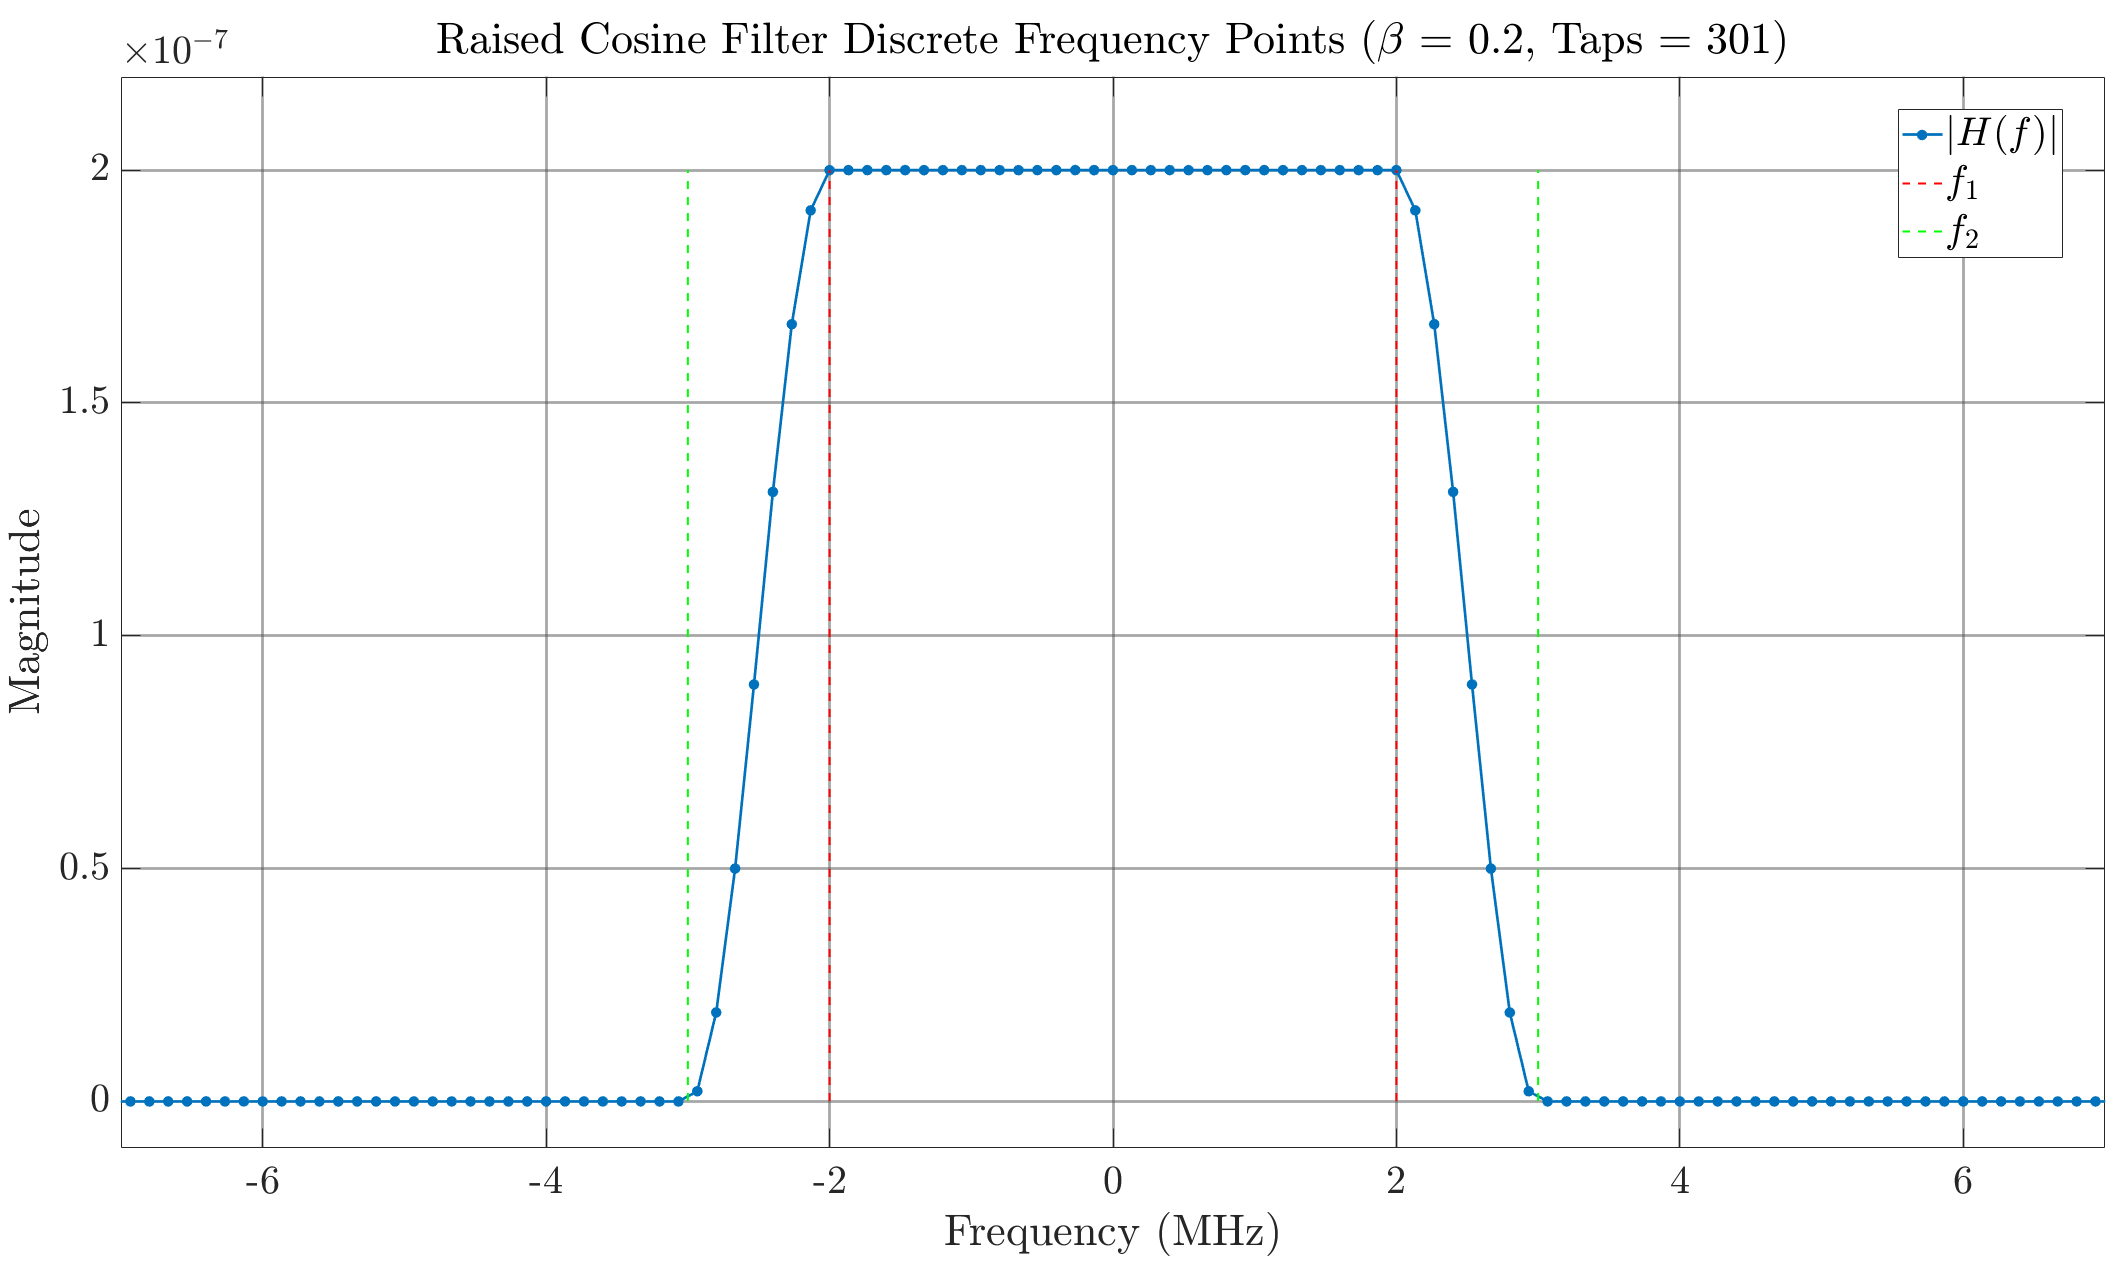
\includegraphics[width=0.9\linewidth]{Images/h-rc-freq} % Ensure 'Images/h-rc-freq' path is correct
	\caption{Raised Cosine Filter Frequency Response ($\beta = 0.2$, $taps = 301$, $OSF = 8$)}
	\label{fig:h-rc-freq}
\end{figure}

In the time domain, the impulse response of the overall RC filter $h(t)$, when sampled at the symbol rate, approximates a Dirac delta function. As shown by the stems representing $h(kT_{symb})$ in Figure \ref{fig:h-rc}, the normalized response is unity at $t=0$ and zero at $t = \pm T_{symb}, \pm 2T_{symb}, \dots$. This property ensures that at the optimal sampling instant for a given symbol, contributions from all other symbols are nullified, thereby eliminating ISI.

\begin{figure}[H]
	\centering
	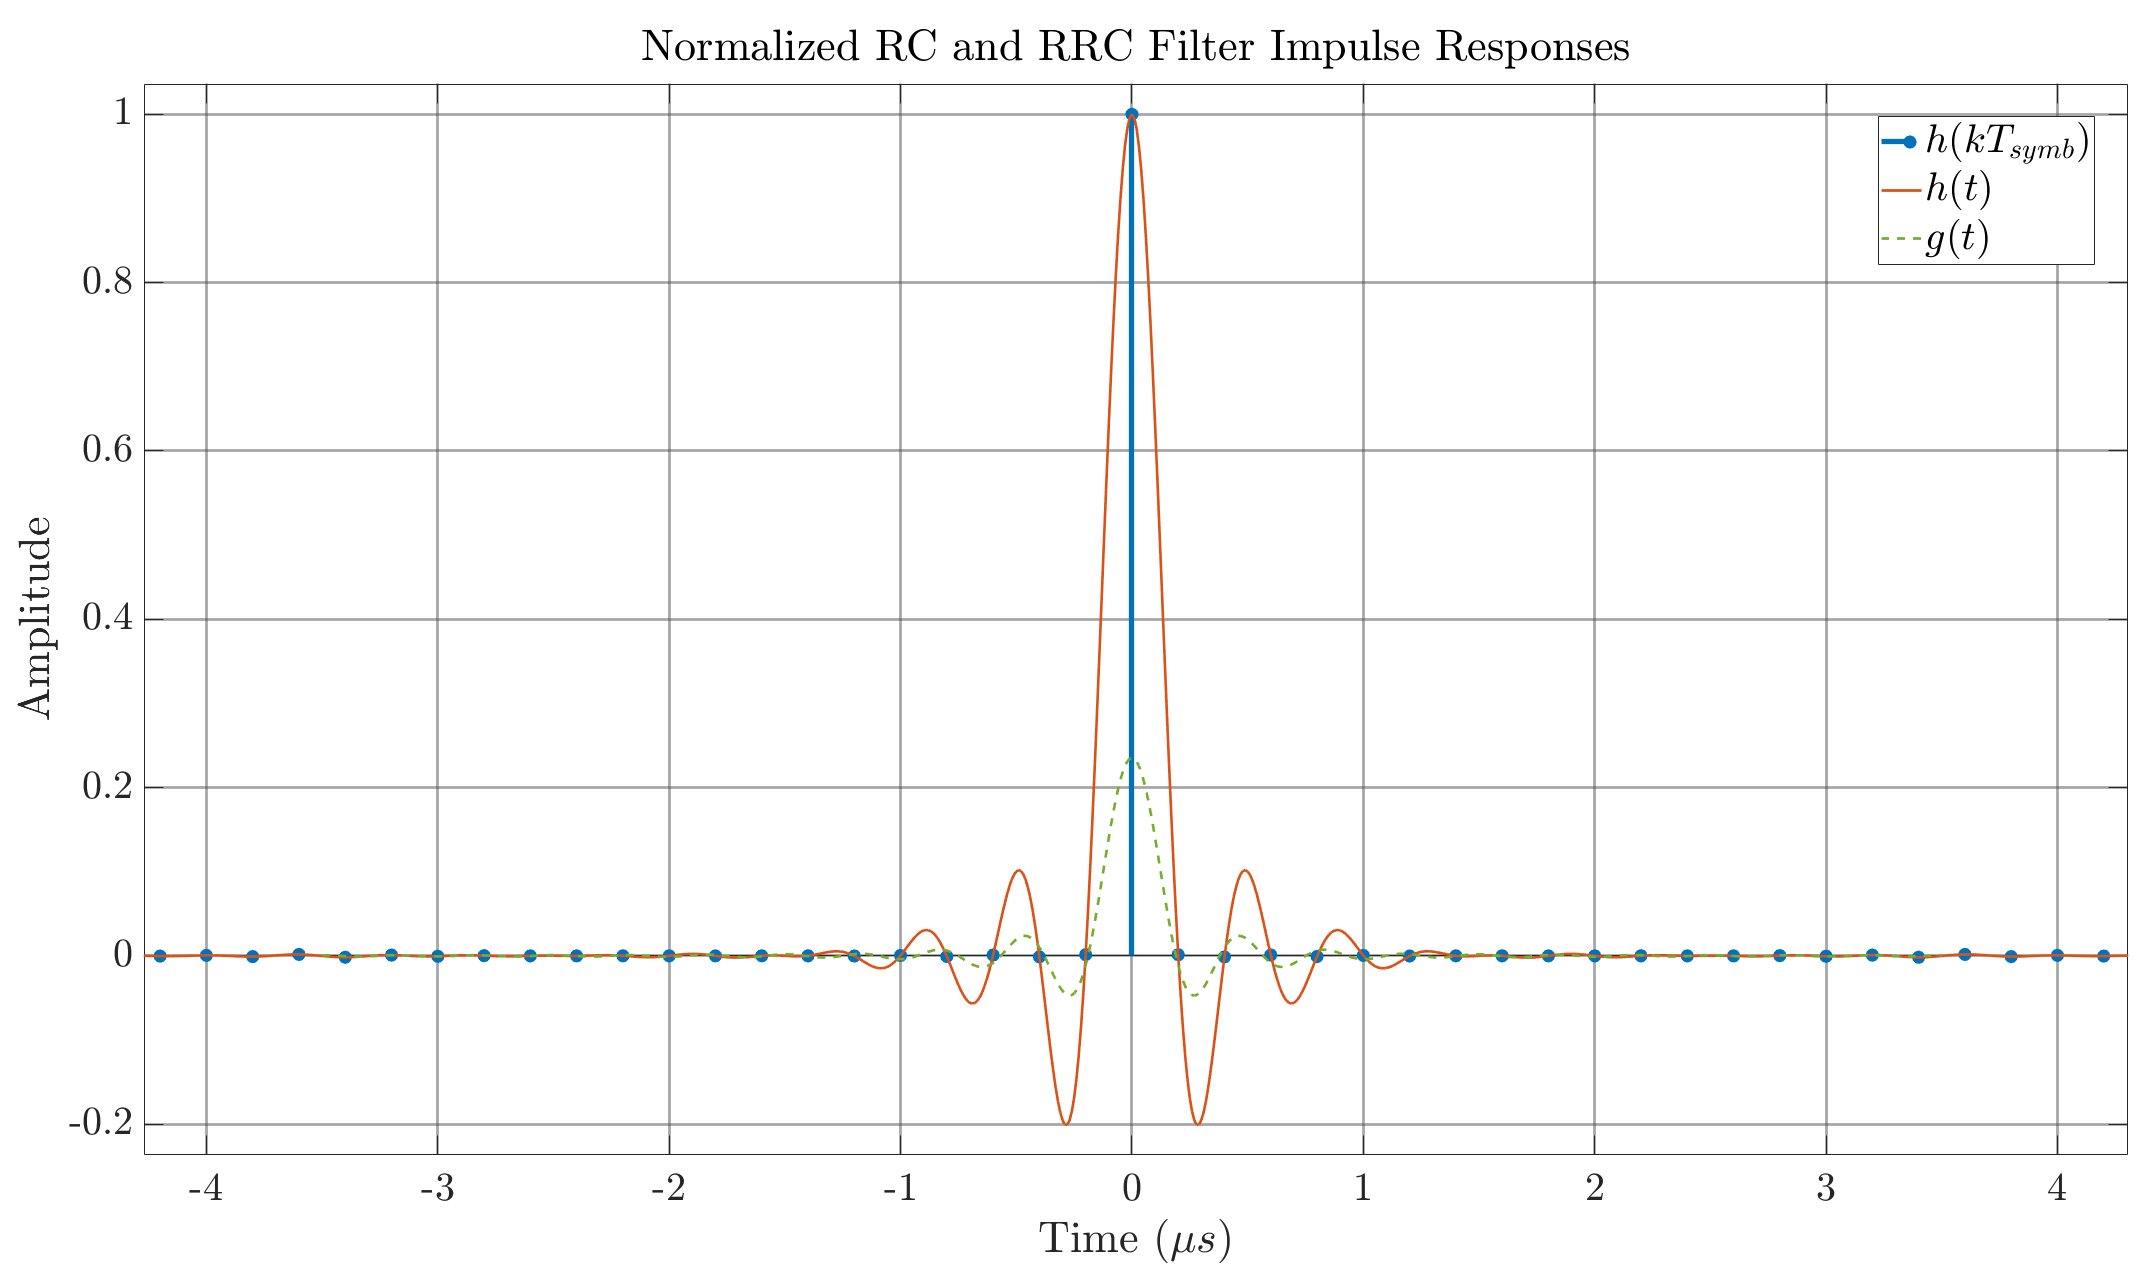
\includegraphics[width=0.9\linewidth]{Images/h-rc} % Ensure 'Images/h-rc' path is correct
	\caption{Normalized RC and RRC filter Impulse Responses}
	\label{fig:h-rc}
\end{figure}

\subsection{Noise Addition and Performance Evaluation}
\textcolor{red}{[LATER]}
\subsection{Questions and Answers}
\textcolor{red}{[LATER]}